O algoritmo de Manacher[1] encontra, para cada posição $i$ da string, o maior
valor de $j$ tal que $s[i-j..i+j]$ é palíndrome, e o maior valor de $j'$ tal que
$s[i-j'+1..i+j']$ é palíndrome (isto é, o algoritmo consegue determinar, para cada
posição da string, o tamanho da substring palíndrome maximal cujo centro ocorre
naquela posição, tanto a de tamanho ímpar ($j$) quanto a de tamanho par ($j'$)). O algoritmo tem complexidade $O(N)$.

A figura abaixo exemplifica a solução para o exemplo dado no enunciado. O
tamanho obtido pelo algoritmo de Manacher é representado em vermelho:

\begin{center}
    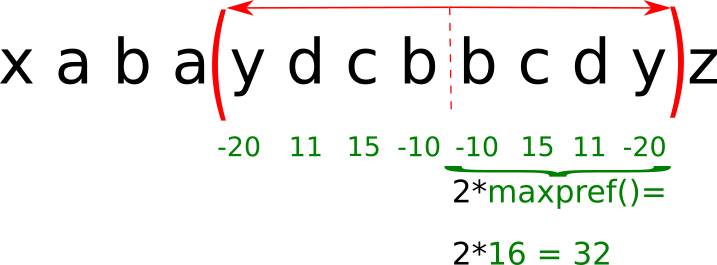
\includegraphics[scale=0.65]{drawkcab/editorial.png}
\end{center}

O próximo passo é determinar o maior valor total possível para cada substring
palindrome maximal. Note que, para substrings de tamanho par, isto é dado por
duas vezes a soma do prefixo de maior soma na segunda metade da substring, e
que, para substrings de tamanho ímpar, é dado por essa soma mais o valor da
letra em seu centro. Na figura exemplificada acima, a resposta é dada por duas vezes a soma do prefixo de maior
soma em $[-10,15,11,-20]$ (que é 16, dado pela soma de $[-10,15,11]$).

Esta soma
pode ser obtida em $O(\lg N)$ através da construção de uma Árvore de
Segmentos adaptada para responder essas consultas, conforme descrito em [2].

Complexidade total: $O(N\lg N)$.

[1] \url{https://cp-algorithms.com/string/manacher.html}

[2] \url{https://www.geeksforgeeks.org/maximum-prefix-sum-given-range/}
